\documentclass[article,12pt, fleqn]{article}

\usepackage{Headers/header}

\title{дизайн документ}
\author{Терехина Полина Сергеевна\\[2mm]
Медведева Ульяна Андреевна \\[2mm]
Чеботова Татьяна Сергеевна \\[2mm]
Игутова Мария Дмитриевна }
\date{Ноябрь - декабрь 2024}
\begin{document}
\maketitle
\begin{center}
    \tableofcontents % Создание оглавления
\end{center}

\newpage
\section{Введение}
\begin{itemize}
    \item Данный документ представляет собой концепцию игры «Super Marmel», описывающую ее\ \ основную\ \ идею,\ \ механику,\ \ жанр,\ \ целевую \ \ аудиторию\ \ и \ \ ключевые \ \ особенности.\\ Документ структурирован по разделам, позволяющим получить полное представление о проекте. 
    \item Ссылки на используемые материалы: 
    \item История изменений документа:
    \item Список авторов: 
    \begin{itemize}
        \item Терехина Полина Сергеевна
        \item Медведева Ульяна Андреевна
        \item Чеботова Татьяна Сергеевна
        \item Игутова Мария Дмитриевна
    \end{itemize}
    \item В документе используются стандартные термины и сокращения, принятые в игровой индустрии. Названия игры, персонажей, мест выделены кавычками.
\end{itemsize}
\section{Концепция}


\subsection{Введение}
"Super Marmel" — это красочный и увлекательный платформер для детей 6+, где игроки управляют одной из четырех девочек-супергероинь, чтобы спасти город "Свит" от злодеев "Аква". Игра предлагает нелинейный геймплей, где игрок самостоятельно выбирает путь и решает головоломки, используя специальные самокаты с яркими фонарями, чтобы ослепить преступников и восстановить мир в городе.

\subsection{Жанр и аудитория}
\par "Super Marmel" относится к жанру 2D-платформер с элементами приключений и головоломок. Игра сочетает динамичные уровни, где важны скорость реакции и точность управления.
\par Целевая аудитория игры — дети от 6 лет и старше. Основное внимание уделено детям младшего и среднего школьного возраста, особенно девочкам, которые могут ассоциировать себя с героинями игры. Тем не менее, увлекательный геймплей и яркая стилистика делают игру интересной для всех любителей казуальных платформеров.
\par Игра подходит для семейного времяпрепровождения и может быть интересна как начинающим, так и опытным игрокам благодаря сочетанию доступного управления и возрастающей сложности уровней.

\subsection{Основные особенности игры}
\begin{itemize}
    \item  Платформер 2D с 5 постепенно усложняющимися уровнями.
    \item Персонаж с базовыми действиями: бег и прыжок.
    \item 3 типа врагов с различными поведением: статичные, бегающие и летающие.
    \item Смерть при столкновении с врагом.
    \item Победа над врагами путем прыжка на них.
    \item Меню с опциями: играть, продолжить, выйти.
    \item Кнопка паузы и клавиша escape для остановки игры и выбора дальнейших действий.
    \item Переход на следующий уровень при победе над всеми врагами и достижении мармеладного мишки.
\end{itemize}

\subsection{Описание игры}
Прославьтесь в эпическом путешествии, где вы берете на себя роль бесстрашной девушки-героя. В этом захватывающем 2D-платформере вас ждет захватывающее испытание с пятью усложняющимися уровнями.\par
Управляйте своей героиней с помощью интуитивно понятных элементов управления бегом и прыжками. Внимательно изучайте каждый уровень, ловко перепрыгивая через препятствия и избегая опасных врагов. \par
Мобилизуйте уникальный талант своей героини в битве. Прыгая на врагов, вы можете победить их и очистить себе путь. Вы должны быть достаточно быстры, чтобы избежать столкновений, так как они могут убить вашу героиню.\par
Пробивайтесь через разнообразные и все более сложные уровни, каждый из которых предлагает уникальные испытания. \par
Присоединяйтесь к отважной девочке-герою в этом захватывающем 2D-платформере, где ловкость, смекалка и отвага станут ключом к победе. Испытайте себя и победите все препятствия, которые встанут на вашем пути!

\subsection{Предпосылки создания}
Рынок игр для мобильных устройств растет, особенно среди более молодой аудитории. Поэтому необходимо создать уникальный продукт, который будет выделяться среди остальных.\par 
В \ \ последние\ \ годы\ \ наблюдается\ \ значительное\ \ увеличение\ \ спроса\ \ на\ \ мобильные\ \ игры. \\ Android и IOS --- наиболее популярные платформы с миллиардами пользователей по всему миру. Это делает их идеальными для запуска новых игровых проектов, особенно для подростковой и детской аудитории. Жанр платформеров остается востребованным благодаря своей доступности и простоте, что важно для выбранной аудитории. Такие игры часто
сочетают элементы приключенией, головоломок и экшена, что добавляет им приквлекательности. \par
Современные игры всё чаще предлагают игрокам разнообразие персонажей, что делает их более привлекательными для широкой аудитории. Возможность выбрать из нескольких девочек-супергероев позволит игрокам проявить индивидуальность и идентифицировать себя с персонажем. \par
"Super Marmel" предлагают комбинацию яркой анимации и динамичного игрового процесса, что соответствует современным тенденциям. Динамика противостояния героев и злодеев стимулирует интерес игроков. Создание злодеев "Аква" дает возможность постепенно развивать сюжет и представлять игрокам различных интересных антагонистов.

\subsection{Платформа}
Игра разрабатывается для Android и iOS. Дополнительное оборудование не потребуется.
Требования:\\[2mm]
\textcolor{white}{.}\hspace{-1cm}\begin{tabular}{|c|c|c|}
    \hline
    Требования & Минимальные & Рекомендуемые\\ \hline
    Операционная система & 64 - битная & 64- битная\\ \hline
    Процессор & 4 ядра & 6-8 ядер\\ \hline
    ОЗУ & не менее 3000 МГц с таймингом 17& 3600 МГц и более с таймингом 16\\
    & и ниже. Объем памяти — 8-16 ГБ &  и ниже. Объем памяти — 16-32 ГБ\\ \hline
    CD-ROM привод & не требуется & не требуется\\ \hline
    Свободное место на HDD &минимум 1ГБ  &минимум 1ГБ \\ \hline
    Видеокарта & Память - 2ГБ & Память - 2ГБ\\ 
    & Частота памяти 5000-6000МГц & Частота памяти 5000-6000МГц \\ \hline
    Звуковая карта &опционально& опционально \\ \hline
    Управление &Клавиатура, мышь & Клавиатура, мышь или геймпад\\ \hline
\end{tabular}\\[2mm]

\section{Функциональная спецификация}

\subsection{Принципы игры}

\subsubsection{Суть игрового процесса}
Super Marmel — это 2D платформер, где игрок управляет одной из четырёх девочек-супергероинь ("Мармеладок"). Цель игры — пробраться через уровни, представляющие собой различные локации вымышленного города Свит, используя самокаты с яркими фонарями, чтобы ослепить и обезвреживать врагов из банды "Аква". Уровни будут включать в себя препятствия, головоломки и сражения с врагами. Удовольствие игрока будет заключаться в динамичном геймплее, преодолении препятствий, решении головоломок и победе над злодеями, а также в возможности выбора персонажа с потенциально уникальными способностями. Возможно добавление коллекционных предметов, открывающих новые элементы кастомизации персонажа или дополнительные уровни.

\subsubsection{Ход игры и сюжет}
Игра начинается с вступительного экрана, представляющего город Свит и команду "Мармеладок". Затем игрок выбирает одного из четырёх персонажей. Каждый уровень представляет собой определённую зону города Свит, заселённую врагами из банды "Аква". Игрок управляет своим персонажем на самокате, используя фонарь для ослепления врагов. Некоторые уровни будут содержать головоломки, требующие использования особенностей окружающей среды или умелого маневрирования. По ходу игры игрок может собирать бонусные предметы (например, усиления для фонаря, дополнительные жизней) и постепенно раскрывает план банды "Аква" по захвату Свита. В конце каждого уровня игрок сталкивается с боссом-злодеем. После победы над всеми боссами и разоблачения плана "Аква", игрок завершает игру. 
\subsection{Физическая модель}
\begin{itemize}
    \item Перемещения: 
    \begin{itemize}
        \item Движение персонажа на самокате осуществляется с помощью стандартных элементов управления (стрелки влево/вправо, прыжок). 
        \item Прыжки подчиняются законам физики, с учётом силы тяжести и высоты прыжка. 
        \item Возможна реализация двойного прыжка или других способностей для персонажей. 
        \end{itemize}
    \item Боевые действия:
    \begin{itemize}
        \item Основное оружие — фонарь на самокате, временно ослепляющий противников. 
        \item Враги имеют определённое время уязвимости после ослепления. 
        \item В игре не будет сложной системы комбо-ударов или спецприемов. 
        \item Противники могут двигаться, наносить урон, иметь различные типы атаки и здоровья. 
    \end{itemize}
    \item Общие формулы:
    \begin{itemize}
        \item Скорость движения: $v = a\cdot t$, где $v$ --- скорость, $a$ --- ускорение, $t$ --- время. 
        \item Высота прыжка: $h = v_0 \cdot t - 0.5\cdot g\cdot t^2$, где $h$ --- высота, $v_0$ --- начальная скорость прыжка, $g$ --- ускорение свободного падения, $t$ --- время полёта.
        \item Повреждения от столкновений: Упрощенная модель, где урон наносится при прямом столкновении с противником в момент уязвимости.
    \end{itemize}
    \item Дополнительные аспекты: 
    \begin{itemize}
        \item Игра будет иметь мультяшную графику с яркими цветами, подчеркивающими контраст между красочным городом и мрачными логовами злодеев. 
        \item Звуковое сопровождение будет соответствовать жанру платформера, с фокусом на веселые мелодии и звуковые эффекты. 
        \item Уровни будут разнообразны по дизайну, с использованием различных платформ, препятствий и головоломок.
    \end{itemize}
\end{itemize}

\subsection{Персонаж игрока}
Игрок управляет одним из четырёх персонажей — девочками-супергероинями, называемыми "Мармеладки". Каждая героиня обладает уникальными особенностями и способностями, что позволяет выбирать персонажа в зависимости от предпочтений игрока. Основное оружие героини — фонарь на самокате, который используется для ослепления врагов. Персонажи обладают базовыми действиями, такими как бег, прыжки, а также могут использовать дополнительные способности, например, двойной прыжок. Героини преодолевают различные препятствия, решают головоломки и сражаются с врагами, сталкиваясь с уникальными вызовами на каждом уровне.

\subsection{Элементы игры}
%---
Оружие: 
    \begin{itemize}
        \item Описание: Основное оружие — фонарь на самокате главных героинь.
        \item Назначение: Служит для ослепления врагов на определенное время, что дает игроку стратегическое преимущество.
        \item Влияние на игровой мир: Ограниченное время уязвимости врагов после ослепления требует от игрока быстроты и точности действий, повышая динамику игры.
        \item Параметры и особенности: 
        \begin{itemize}
            \item Временное действие ослепления.
            \item Нет сложных комбо-ударов, что упрощает механику боя.
            \item Интегрирована в механики передвижения, так как фонарь использован на самокате.
        \end{itemize}
    \end{itemize}
%----
Главные персонажи: 
    \begin{itemize}
        \item Описание: Главными персонажами являются четыре девочки-супергероини, каждая из которых обладает уникальными способностями и умениями. Это позволяет игроку выбирать персонажа, который наиболее соответствует его стилю игры.
        \item Назначение: Главные персонажи служат основным инструментом игрока для взаимодействия с игровым миром, преодоления препятствий, решения головоломок и борьбы с врагам
        \item Влияние на игровой мир: Каждая героиня предоставляет уникальный опыт прохождения благодаря своим способностям. Выбор персонажа может влиять на легкость преодоления определенных уровней.
        \item Параметры и особенности: 
        \begin{itemize}
            \item Базовые действия: бег, прыжки.
            \item Каждая героиня имеет свои характеристики, такие как скорость, ловкость и др.
        \end{itemize}
    \end{itemize}
%---
Враги: 
    \begin{itemize}
        \item Описание: Враги представляют собой барьеры для героинь, мешая им достигать цели.
        \item Назначение: Создают вызов игроку, требующий использования способности персонажей для их преодоления.
        \item Влияние на игровой мир: Сложность врагов меняется на разных уровнях, поэтому игроку необходимо адаптировать стратегии.
        \item Параметры и особенности: 
        \begin{itemize}
            \item Способны наносить урон.
            \item Уязвимы к ослеплению на определенное время.
        \end{itemize}
    \end{itemize}
%---
Транспортные средства:
\begin{itemize}
        \item Описание: Самокат — средство передвижения главных героев в игре, представляющее собой стилизованный транспорт.
        \item Назначение: Самокат обеспечивает быстрый и удобный способ передвижения по игровому миру, наделяет героинь скоростью и ловкостью, позволяет им преодолевать расстояния и исследовать локации. Самокат имеет фонарь, удлинение света которого ослепляет врагов.
        \item Влияние на игровой мир: Самокат значительно ускоряет передвижение героев, расширяя возможности исследования игрового мира и увеличивая темп игры. Самокат может изменять тактику прохождения игры, предоставляя возможность ослеплять врагов.
        \item Параметры и особенности: 
        \begin{itemize}
            \item Каждая из героинь имеет свой, непохожий на других самокат.
             \item Ускорение героинь.
              \item Наличие фонаря, способного ослеплять врагов.
        \end{itemize}
    \end{itemize}
%---
Карты и уровни: 
    \begin{itemize}
        \item Описание: Каждый уровень представляет собой уникальный набор испытаний, включающий головоломки и препятствия.
        \item Назначение: Составляют главные объекты игрового мира, позволяя развиваться истории игры и взаимодействовать с персонажами
        \item Влияние на игровой мир: Уровни содержат различные элементы, которые героини могут использовать для решения головоломок или обхода преград.
        \item Параметры и особенности: 
        \begin{itemize}
            \item Различные уровни сложности
        \end{itemize}
    \end{itemize}
%---
Строения: 
    \begin{itemize}
        \item Описание: Мармеладный Медведь – это крупная, яркая, выполненная в стиле мультяшной стилизации фигура медведя, изготовленная из розового, полупрозрачного мармелада. 
        \item Назначение:Мармеладный Медведь служит основным средством перемещения героини между уровнями игры. Взаимодействие с ним инициирует анимацию перехода между уровнями, создавая эффект плавного “перетекания” из одной игровой среды в другую.
        \item Влияние на игровой мир: Медведь служит ярким порталом между уровнями, для его активации героине необходимо убить всех врагов.
        \item Параметры и особенности: 
        \begin{itemize}
            \item Довольно крупный, чтобы быть заметным на экране и служить явным указателем на точку перехода.
            \item Работает только при обезвреживании всех врагов на уровне.
        \end{itemize}
    \end{itemize}


\subsection{Искуственный интеллект}
Искусственный интеллект (AI) в игре Super Marmel отвечает за поведение врагов, которые включают несколько типов: статичные, бегающие и летающие. AI врагов направлен на обеспечение динамичного взаимодействия с игроком, а также на создание интересных и сложных ситуаций. Враги могут двигаться по заранее заданным траекториям, а также реагировать на действия игрока, например, атаковать, когда находятся в пределах досягаемости, или избегать ослепления фонарём. Некоторые враги будут следовать за героиней, другие — охранять определенные зоны, а третьи — могут двигаться хаотично, создавая дополнительные трудности для игрока. Основной задачей AI является поддержание баланса сложности и обеспечивание непредсказуемости, чтобы игрок чувствовал вызов, но не перегружался.

\subsection{Многопользовательский режим}
\subsection{Интерфейс пользователя}
\subsubsection{Блок-схема}
\subsubsection{Функциональное описание и управление}
\subsubsection{Объекты интерфеса пользователя}
\subsection{Графика и Видео}
\subsubsection{Общее описание}
\begin{itemize}
    \item Техническое исполнение: 
            2D платформер с постепенно усложняющимися уровнями. Игра разрабатывается для Android и iOS.
    \item Стилистика, атмосфера и палитра: 
            Яркая, красочная, мультяшная стилистика. Палитра состоит из насыщенных, позитивных цветов, контрастирующих с более темными оттенками, используемыми для обозначения мест обитания злодеев. Атмосфера должна передавать ощущение веселья и приключений, но с легким налетом интриги и напряжения в местах, контролируемых "Аква".
    \item Другие общие сведения: 
            Графика должна быть достаточно простой, чтобы обеспечить плавную работу игры на устройствах с разными характеристиками. Оптимизация для мобильных платформ – приоритетная задача.
\end{itemize}
\subsubsection{Двумерная графика и анимация}
\begin{itemize}
    \item Интерфейс: Простой и интуитивно понятный интерфейс, адаптированный под сенсорное управление. Яркие иконки, четкий шрифт. Отображение здоровья персонажа, индикатор прогресса, карта уровня (мини-карта) и элементы управления (кнопки прыжка, движения, использования самоката).
    \item Эффекты:
    \begin{itemize}
        \item Свет от самокатов: Яркие вспышки света, ослепляющие врагов (возможно, с использованием частичного затемнения экрана).
        \item Эффекты разрушения: Упрощенные эффекты разрушения объектов (рассыпание конфет, обломки зданий), без излишней детализации.
        \item Частицы: Использование частиц для создания эффекта движения (пыль, искры).
        \item Звуковые эффекты: Сопровождение эффектов звуковыми сигналами (вспышка света, взрыв).
    \end{itemize}

    \item Персонажи, строения и юниты:
    \begin{itemize}
        \item Главные героини: Четыре уникальных персонажа с выразительной анимацией (бег, прыжки, использование самокатов). Дизайн персонажей должен быть милым и привлекательным для целевой аудитории (6+).
        \begin{figure}[ht]
            \centering
            \begin{minipage}[b]{0.25\textwidth}
                \center{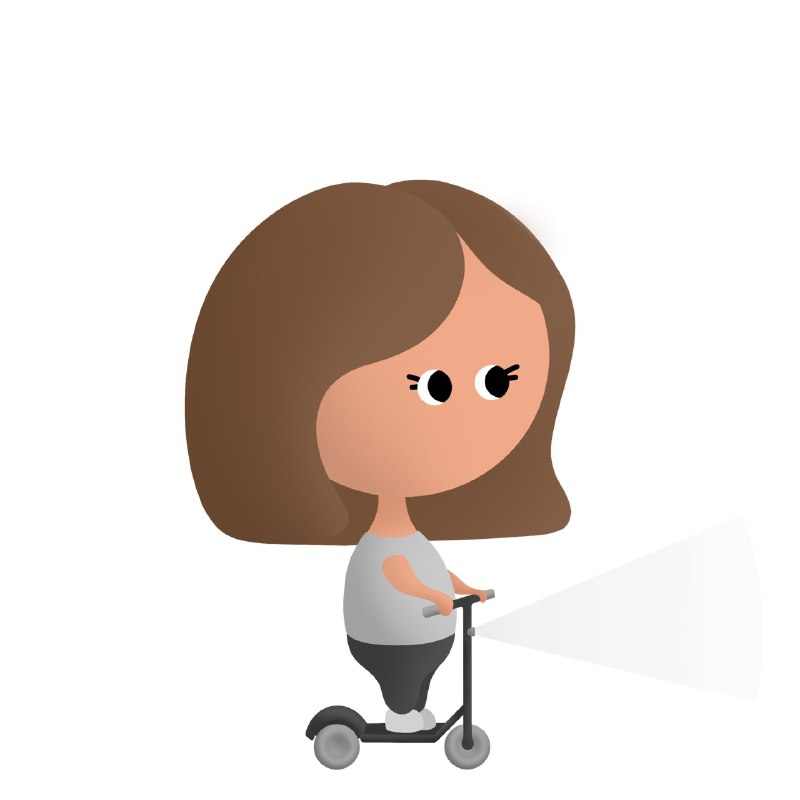
\includegraphics[width=\textwidth]{24-25/марм1.jpeg}}
            \end{minipage}\hfill
            \begin{minipage}[b]{0.25\textwidth}
                \center{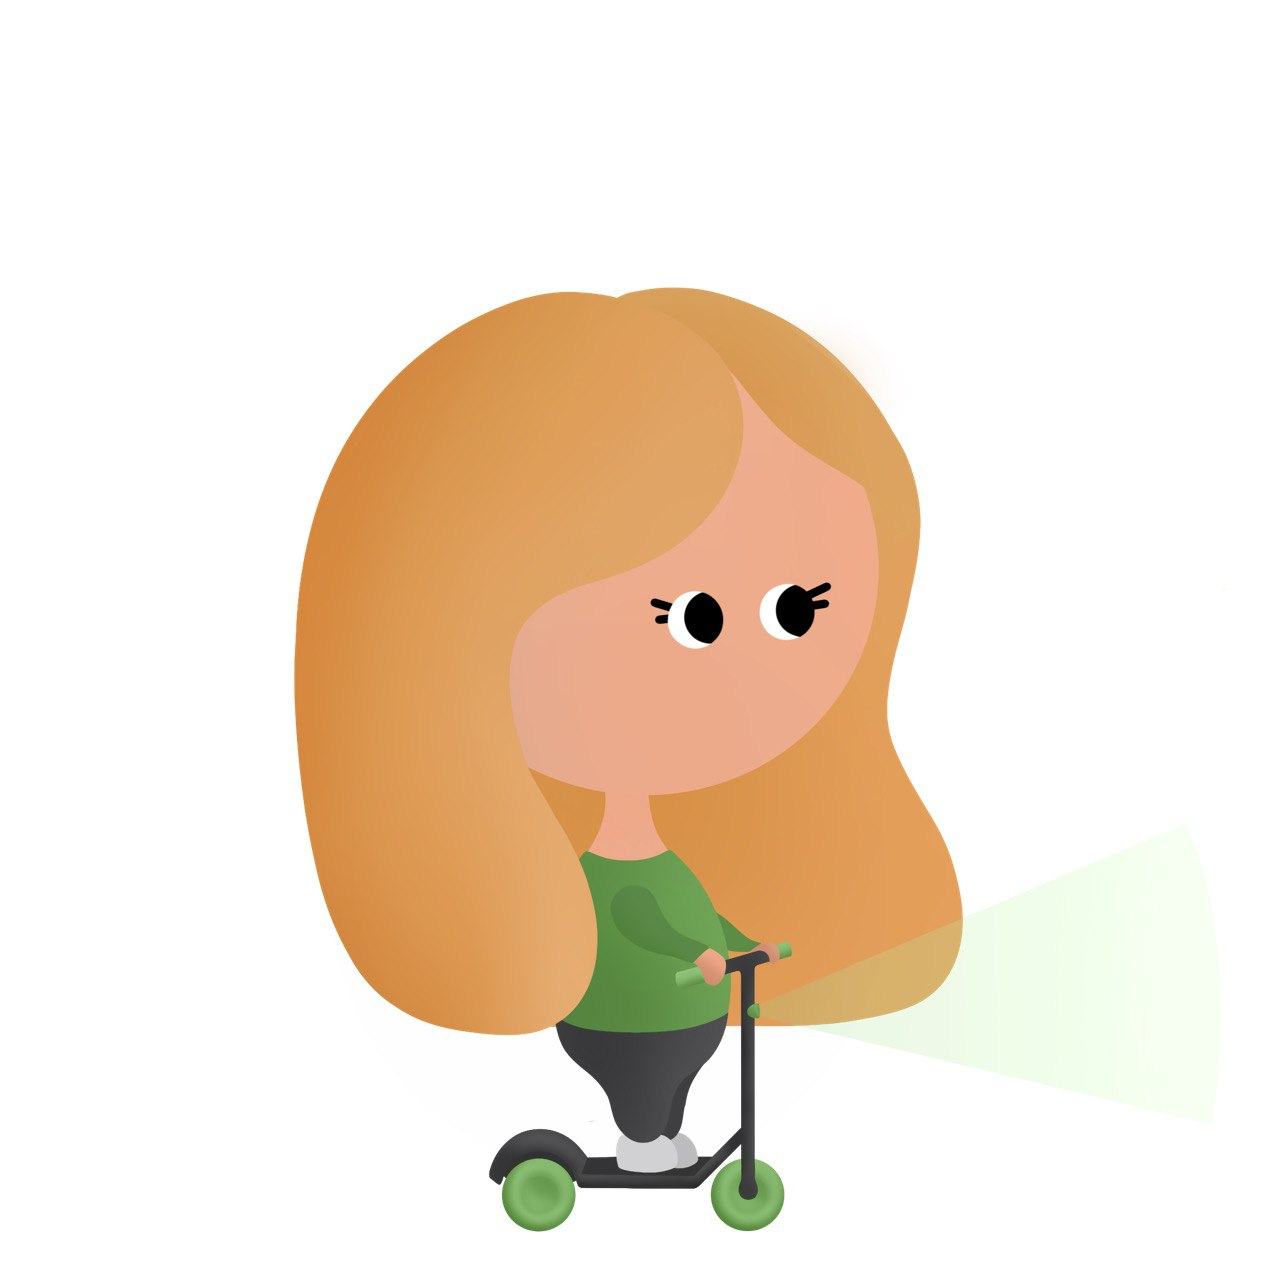
\includegraphics[width=\textwidth]{24-25/марм2.jpeg}}
            \end{minipage}\hfill
            \begin{minipage}[b]{0.25\textwidth}
                \center{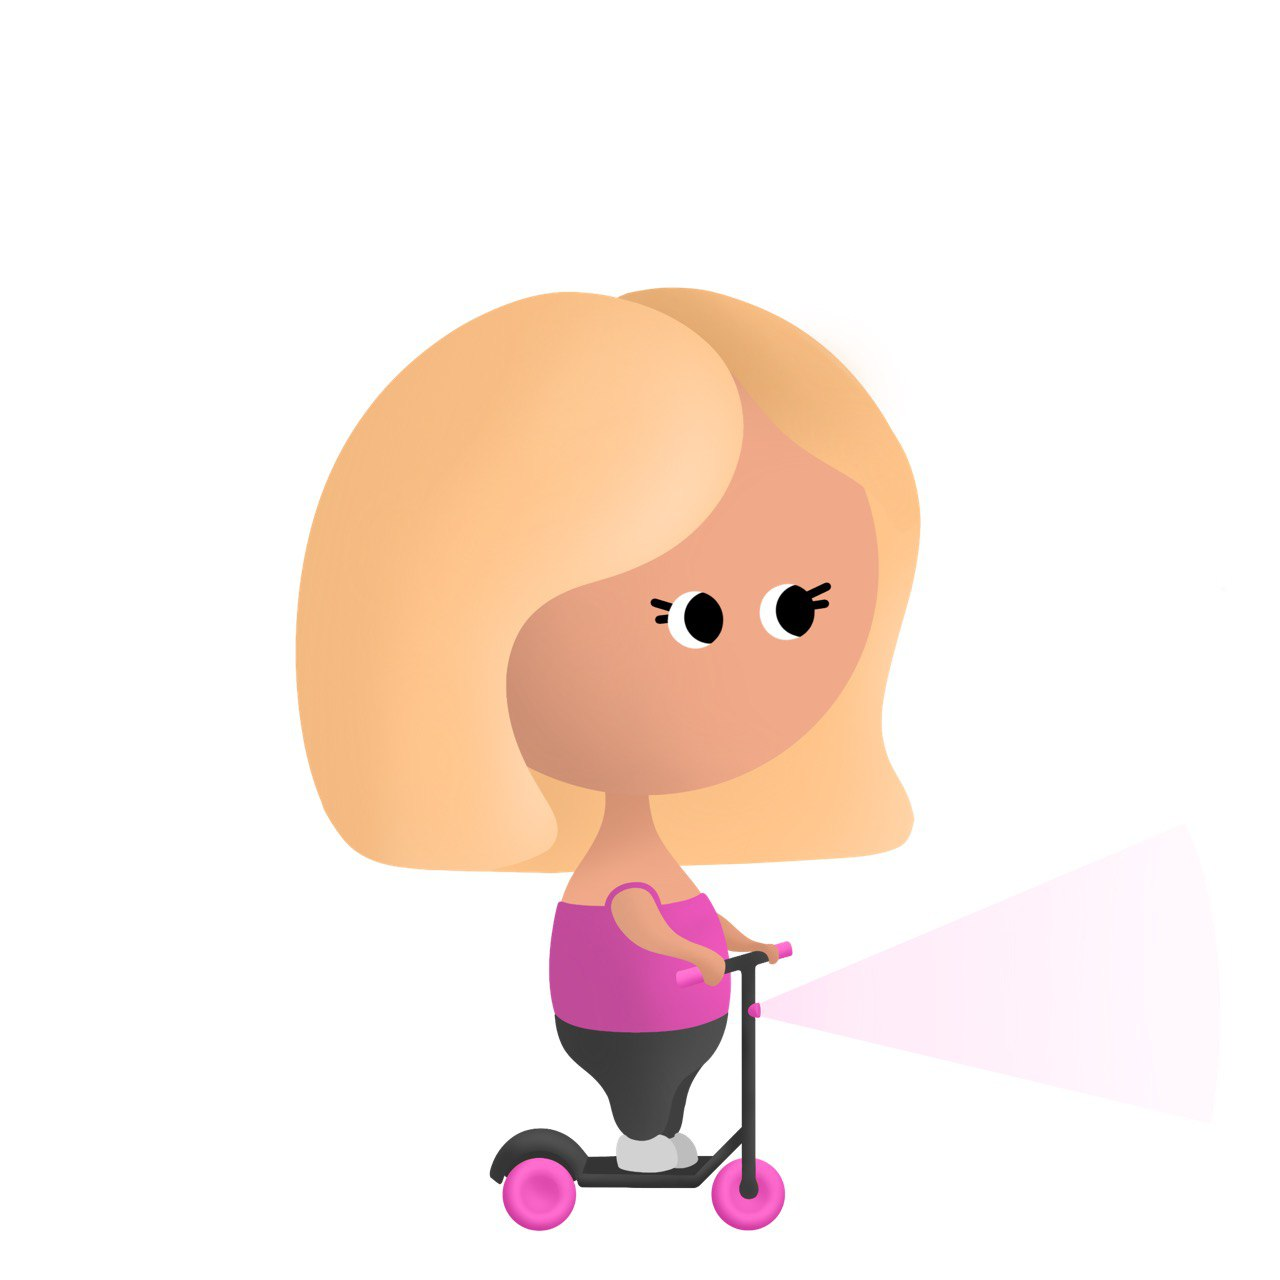
\includegraphics[width=\textwidth]{24-25/марм3.jpeg}}
            \end{minipage}\hfill
            \begin{minipage}[b]{0.25\textwidth}
                \center{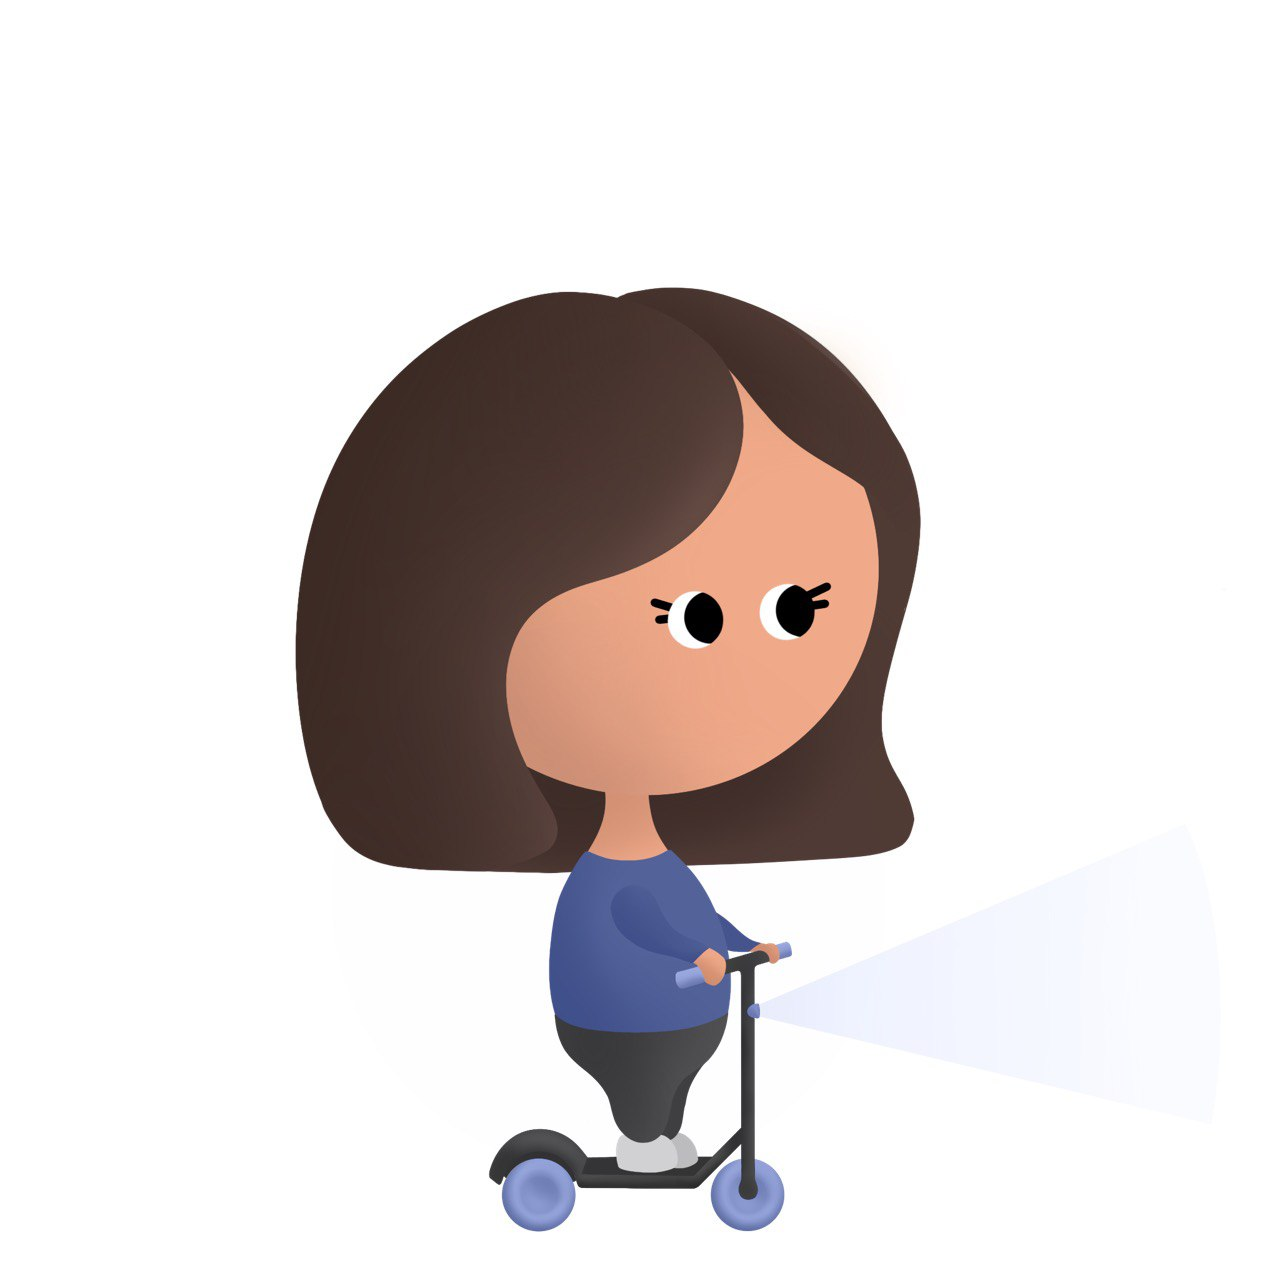
\includegraphics[width=\textwidth]{24-25/марм4.jpeg}}
            \end{minipage}\hfill
            \caption{Главные героини.}
        \end{figure}
        \item Злодеи: Четыре злодея с собственным уникальным дизайном, отражающим их природу банды из маленького городка. Анимация должна соответствовать их роли.
        \begin{figure}[ht]
            \centering
            \begin{minipage}[b]{0.25\textwidth}
                \center{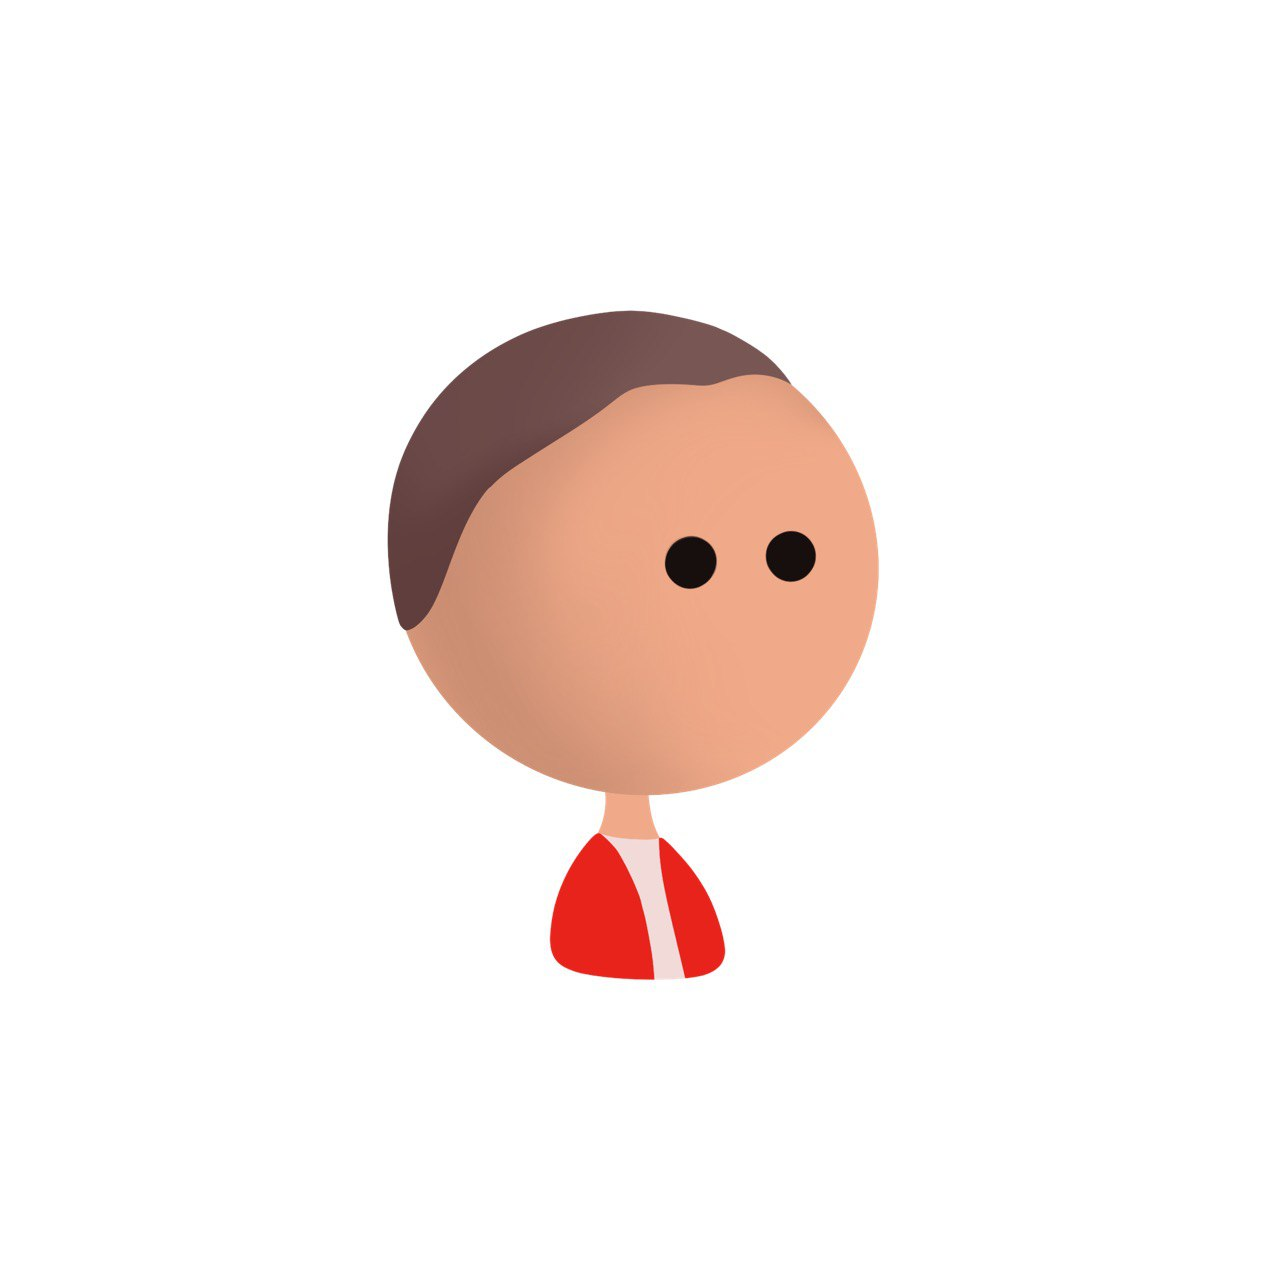
\includegraphics[width=\textwidth]{24-25/аква1.jpeg}}
            \end{minipage}\hfill
            \begin{minipage}[b]{0.25\textwidth}
                \center{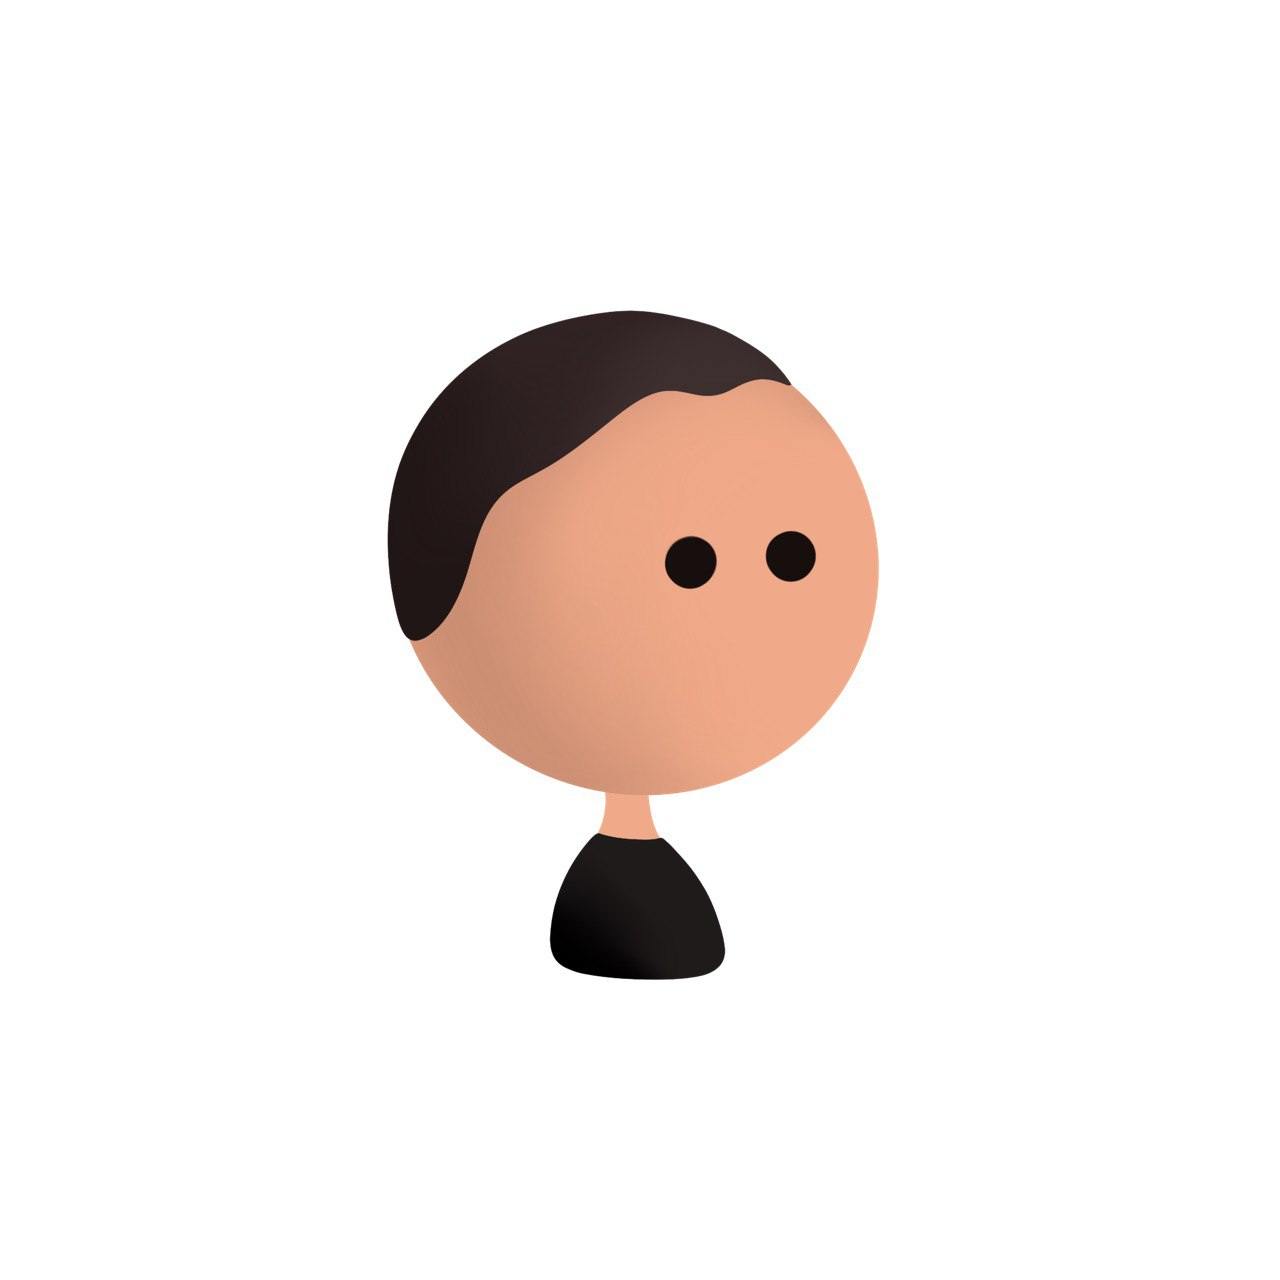
\includegraphics[width=\textwidth]{24-25/аква2.jpeg}}
            \end{minipage}\hfill
            \begin{minipage}[b]{0.25\textwidth}
                \center{
\includegraphics[width=\textwidth]{24-25/аква3.jpeg}}
            \end{minipage}\hfill
            \begin{minipage}[b]{0.25\textwidth}
                \center{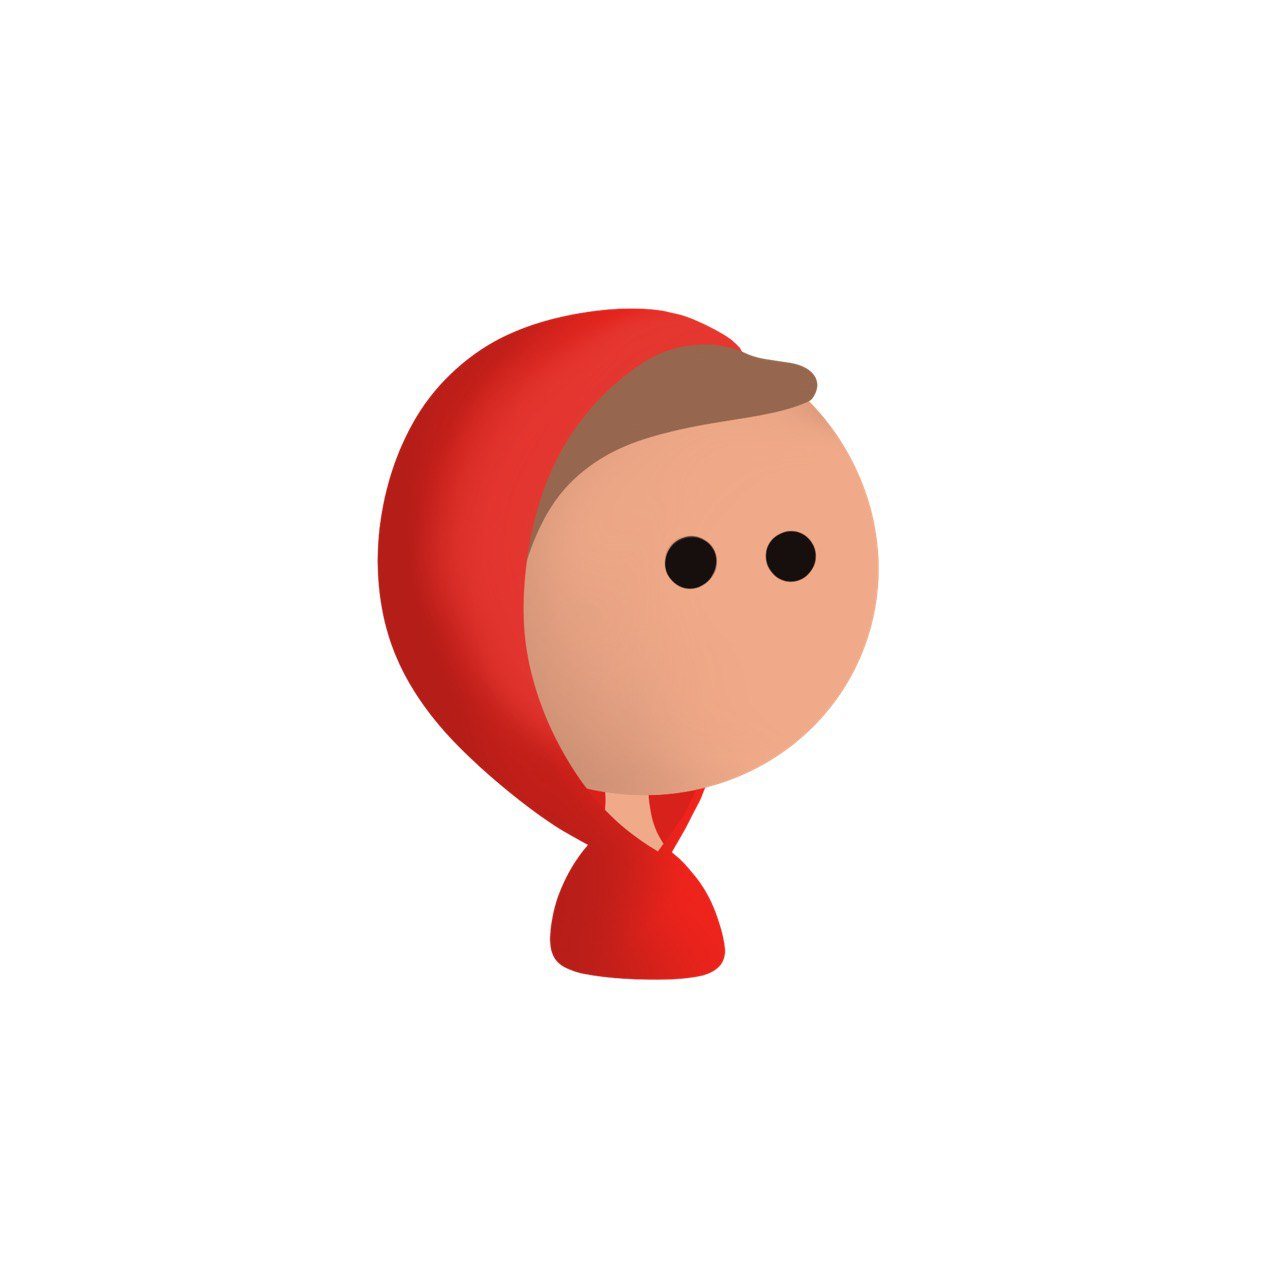
\includegraphics[width=\textwidth]{24-25/аква4.jpeg}}
            \end{minipage}\hfill
            \caption{Злодеи.}
        \end{figure}
        \item Строения: Яркие, красочные здания в стиле мультяшного города. Простые геометрические формы, без излишней детализации.

        \item Статические объекты: Различные элементы городских пейзажей. Очертания города на фоне, сладкие деревья(леденцы).
         \begin{figure}[ht]
            \centering
            \begin{minipage}[b]{0.3\textwidth}
                \center{
\includegraphics[width=\textwidth]{24-25/городсвет.jpeg}}
            \end{minipage}\hfill
            \begin{minipage}[b]{0.3\textwidth}
                \center{
\includegraphics[width=\textwidth]{24-25/вид свет.jpeg}}
            \end{minipage}
            \caption{}
        \end{figure}
    \end{itemize}
    \item Игровой мир (ландшафты и статические объекты):
    \begin{itemize}
        \item Улицы: Разнообразные улицы города Свит, от широких проспектов до узких переулков. Использование различных текстур и объектов для создания интересного игрового пространства.
        \item Зоны врагов: Темные и мрачные зоны, контролируемые злодеями. Использование более темной палитры цветов и специфичных объектов.
        \begin{figure}[ht]
            \centering
            \begin{minipage}[b]{0.3\textwidth}
                \center{
\includegraphics[width=\textwidth]{24-25/вид тем.jpeg}}
            \end{minipage}\hfill
            \begin{minipage}[b]{0.3\textwidth}
                \center{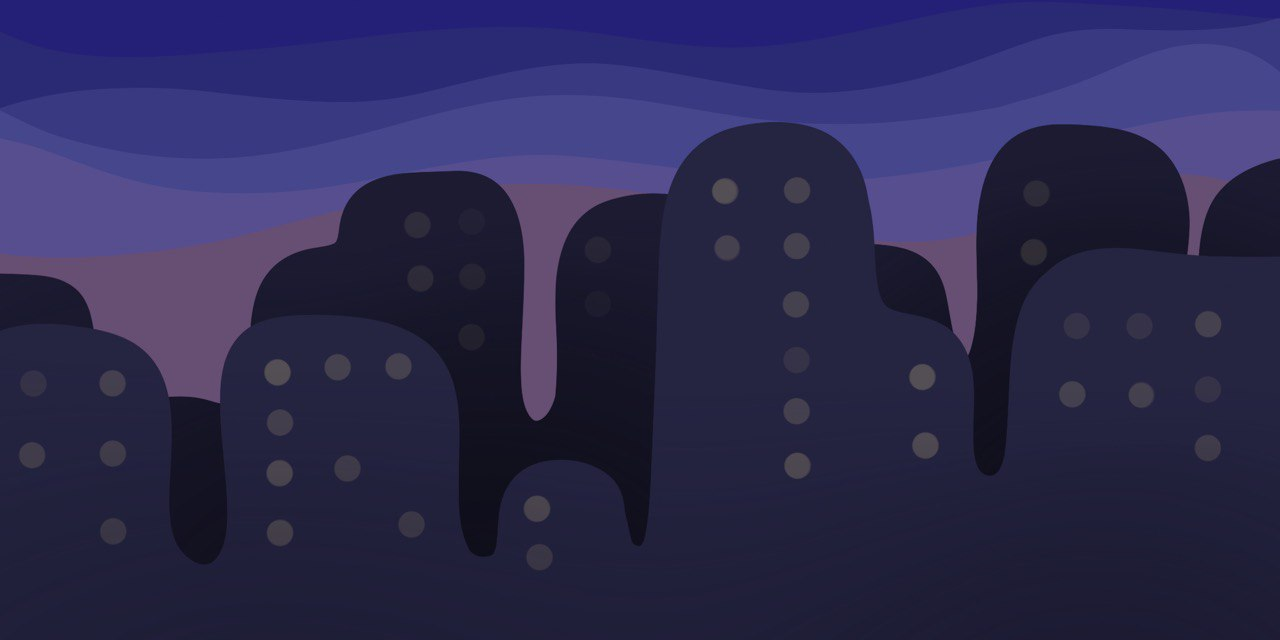
\includegraphics[width=\textwidth]{24-25/городтем.jpeg}}
            \end{minipage}
            \caption{}
        \end{figure}
        \item Разнообразие: Разнообразные локации, чтобы не было монотонности. Некоторые уровни могут иметь вертикальные платформы, другие — скрытые проходы.
        \begin{figure}[ht]
            \centering
            \begin{minipage}[b]{0.3\textwidth}
                \center{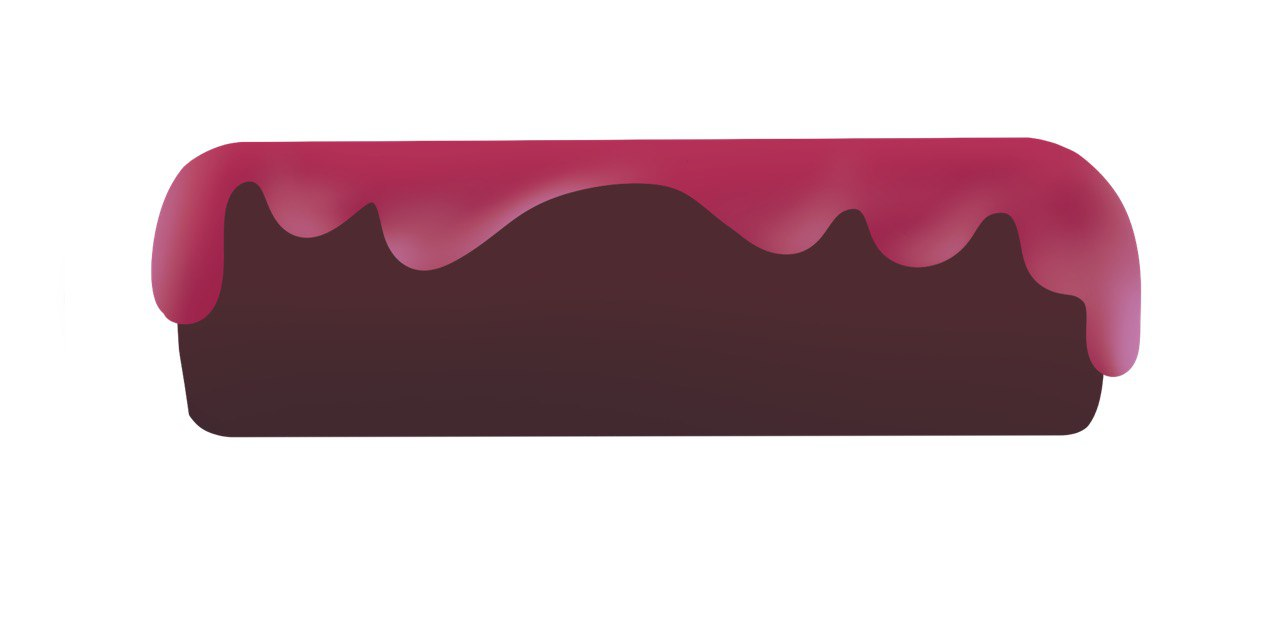
\includegraphics[width=\textwidth]{24-25/платформа.jpeg}}
            \end{minipage}\hfill
            \begin{minipage}[b]{0.3\textwidth}
                \center{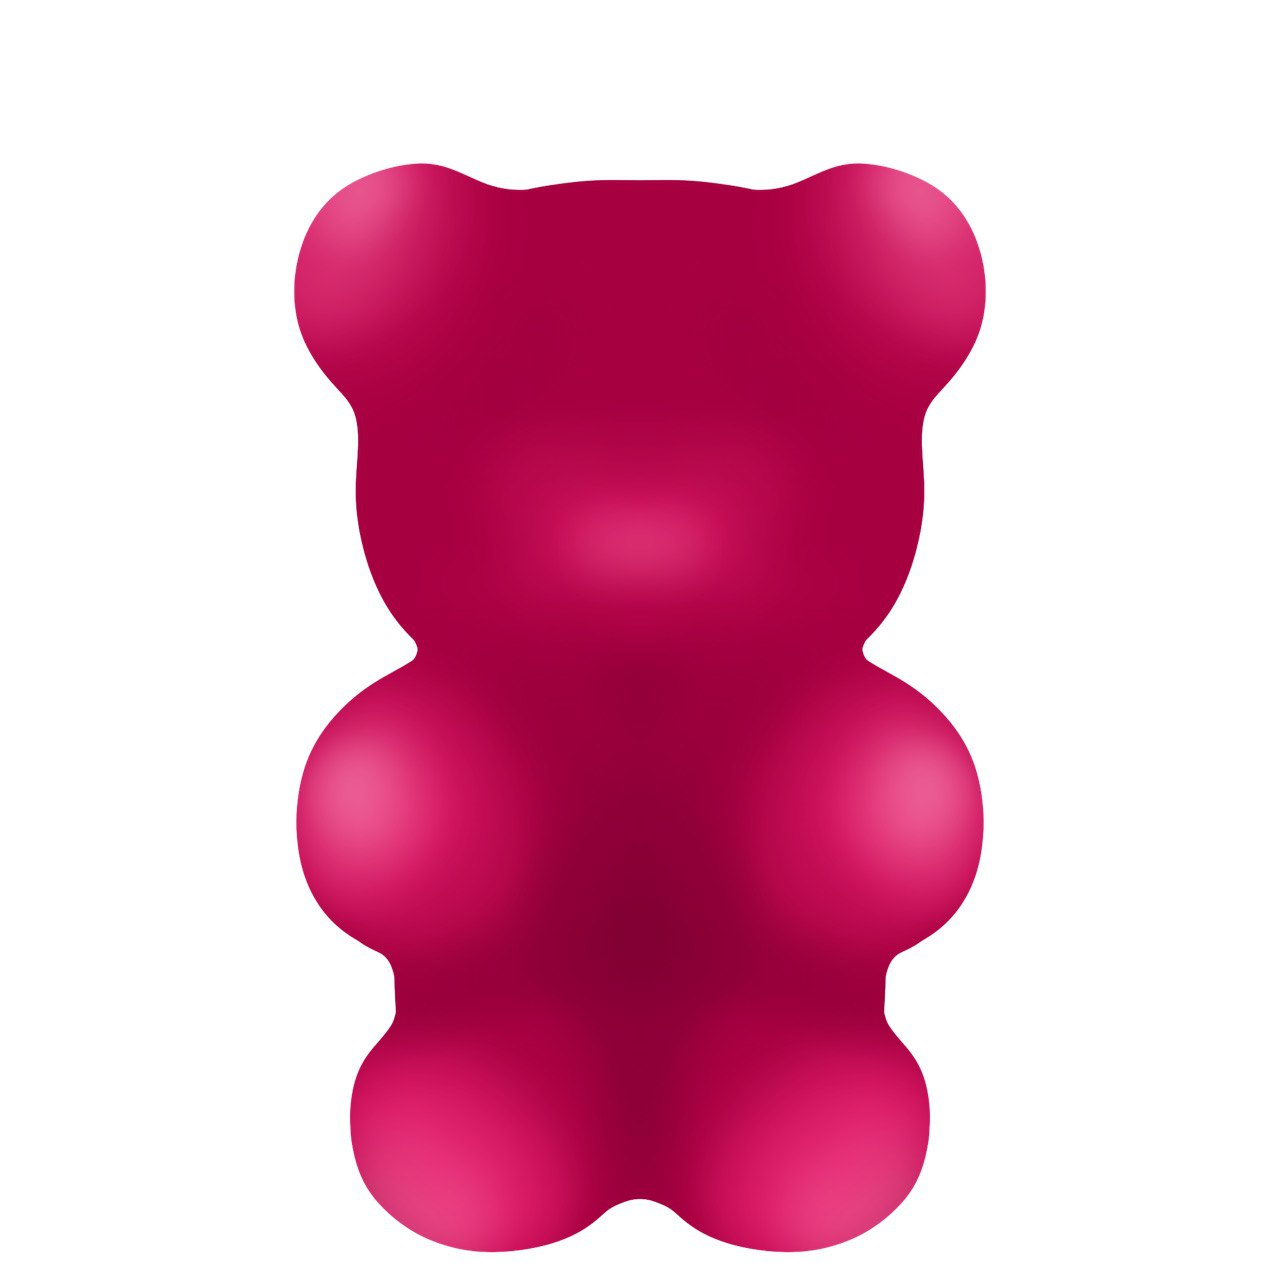
\includegraphics[width=\textwidth]{24-25/дверь.jpeg}}
            \end{minipage}
            \caption{}
        \end{figure}
    \end{itemize}
\end{itemize}
\subsubsection{Трехмерная графика и описание}
\subsubsection{Анимационные вставки}
\subsection{Звуки и музыка}
\subsubsection{Общее описание}
\subsubsection{Звук и звуковые эффекты}
\subsubsection{Музыка}
\subsection{Описание уровней}
\subsubsection{Общее описание дизайна уровней}
\subsubsection{Диаграмма взаимного расположения уровней}
\subsubsection{График введения новых объектов}
\section{Контакты}
\end{document}
